%!TEX root = draft.tex
\section{Stacks With Fixed Pop Commit Points}\label{sec:stacks}

While the abstract queue implementation in Section~\ref{sec:queues} can be adapted to stacks~\footnote{The only modification is that the linearization point $lin(pop,d,k)$ with $d\neq{\tt EMPTY}$ is enabled only if $k$ is added by a push which is maximal in the happens-before order stored in the state.}, it can not simulate (through forward simulations) existing stack implementations like the Time-stamped Stack~\cite{DBLP:conf/popl/DoddsHK15} where the linearization points of the pop operations are not fixed. In this section, we define an abstract implementation which simulates such implementations provided that the point in time where the return value of a pop operation is determined corresponds to a fixed action. To demonstrate the use of this abstract implementation we provide a correctness proof for a simplified version of Time-Stamped Stack that preserves its most complex behaviors.

\subsection{Abstract stack implementation}


\begin{wrapfigure}{l}{5.4cm}
\vspace{-11mm}
\begin{lstlisting}
struct Node{
  int data;
  int ts;
  Node* next;
  boolean taken;
};
Node* pools[maxThreads];
int TS = 0;   

void push(int x) {
  Node* n = new Node(x,MAX_INT,
                        null,false);
  n->next = pools[myTID];
  pools[myTID] = n;
  int i = TS++;
  n->ts = i;
}
int pop() {
 boolean success = false;
 int maxTS = -1;
 Node* youngest = null;
 while ( !success ) {
   maxTS = -1; youngest = null;
   for(int i=0; i<maxThreads; i++){
     Node* n = pools[i];
     while (n->taken && n->next != n)
       n = n->next;
     if(maxTS < n->ts) {
       maxTS = n->ts; youngest = n;
     }
   }
   if (youngest != null)
     success=CAS(youngest->taken,
                       false,true);
 }
 return youngest->data;
}
\end{lstlisting}
\vspace{-6mm}
\caption{Time-Stamped Stack. We assume that every statement is atomic.}
\label{fig:TimeStamped}
\vspace{-8mm}
\end{wrapfigure}
We explain the meaning of the commit points on a simplified version of the Time-Stamped Stack~\cite{DBLP:conf/popl/DoddsHK15} ($\mathit{TSS}$, for short) given in Figure~\ref{fig:TimeStamped}. This stack implementation maintains a vector of singly-linked lists, one for each thread, where list nodes contain a data value (field {\tt data}), a timestamp (field {\tt ts}), the next pointer (field {\tt next}), and a boolean flag indicating whether the node represents a value removed from the stack (field {\tt taken}). Initially, each list contains a sentinel dummy node pointing to itself with timestamp $-1$ and the flag {\tt taken} set to {\tt false}.

Pushing a value to the stack proceeds in several steps: adding a node with maximal timestamp in the list associated to the thread executing the push (given by the special variable {\tt myTID}), asking for a new timestamp (given by the value of the shared integer {\tt TS}), and updating the timestamp of the added node. Popping a value from the stack consists in traversing all the lists, finding the first element which doesn't represent a removed value (i.e., {\tt taken} is {\tt false}) in each list, and selecting the element with the maximal timestamp. A compare-and-swap (CAS) is used to set the {\tt taken} flag of this element to {\tt true}. The procedure restarts if the CAS fails.

\begin{figure}[t]
\centering
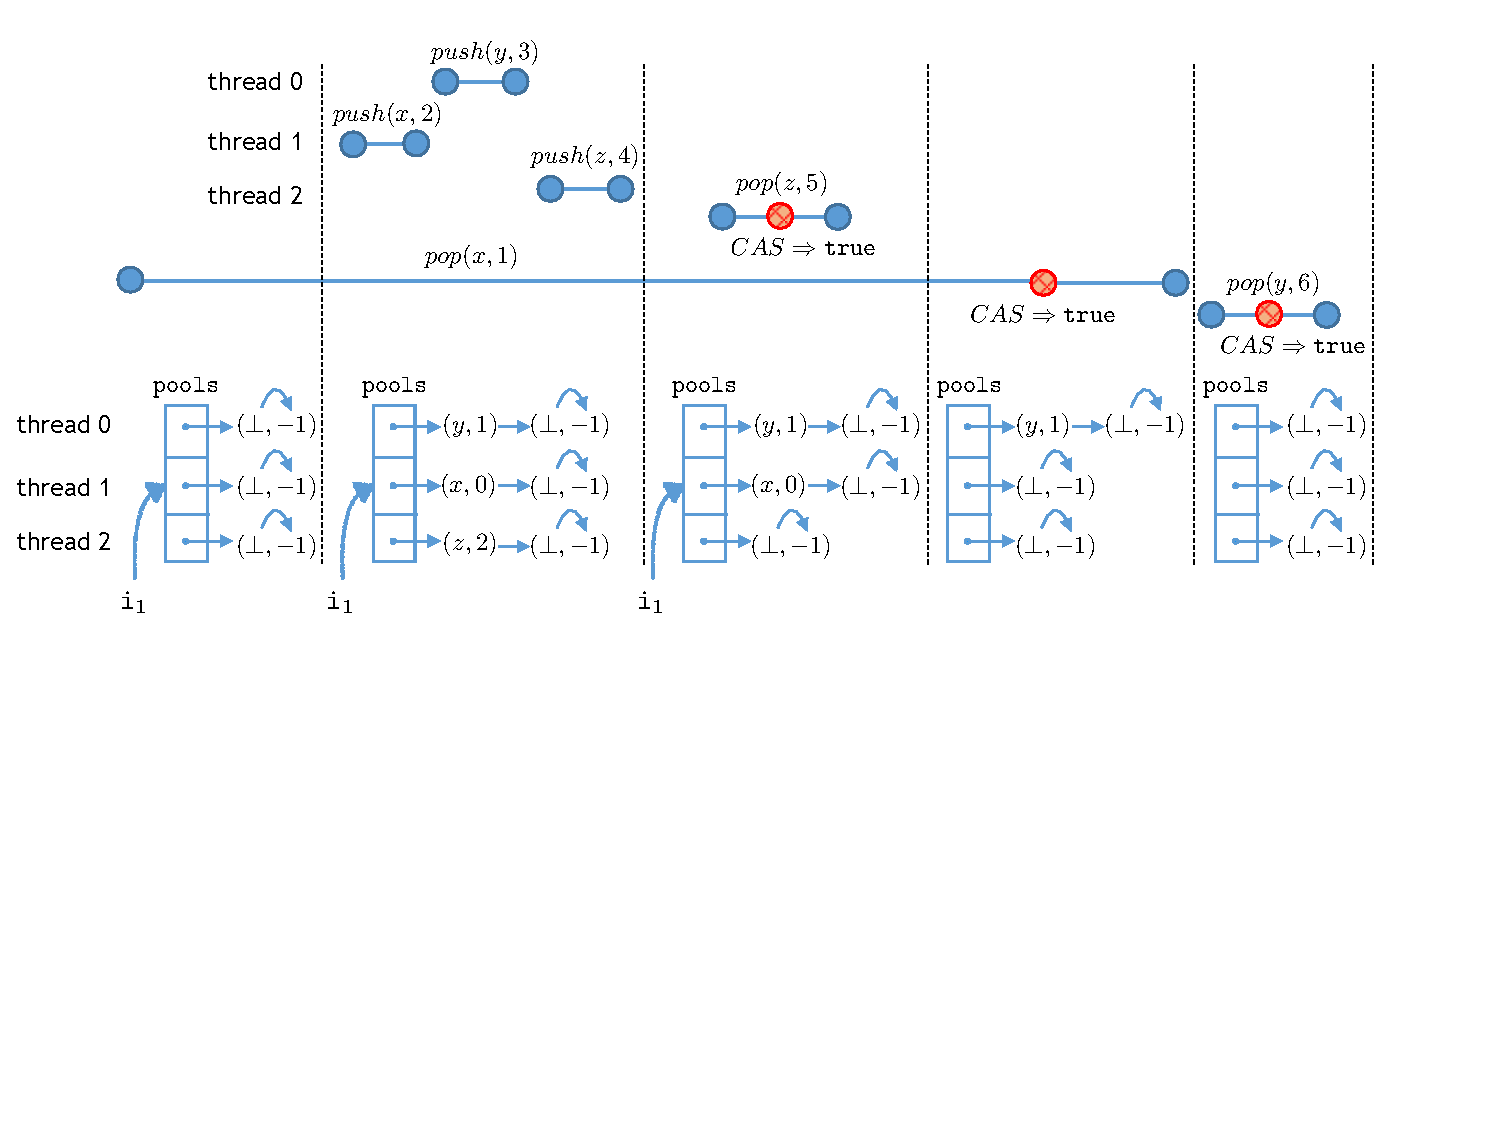
\includegraphics[width=11cm]{fig-timeStamp.pdf}
\vspace{-4.5mm}
\caption{An execution of the Time-Stamped Stack. An operation is pictured by a line delimited by two circles denoting the call and respectively, the return action. Pop operations with identifier $k$ and removing value $d$ are denoted by $pop(d,k)$ and their representation includes another circle to represent a CAS returning {\tt true} which is the commit point of that operation. The state of the library after an execution prefix delimited at the right by a dotted line is pictured in the bottom part (the picture immediately to the left of the dotted line). A pair $(d,t)$ for some value $d$ and integer $t$ represents a list node with ${\tt data}=d$ and ${\tt ts}=t$, and ${\tt i}_1$ denotes the value of {\tt i} in the pop operation with identifier 1. We omit the nodes where {\tt taken} is set to {\tt true}.}
\label{fig:commit}
\vspace{-7mm}
\end{figure}


The push operations don't have a fixed linearization point because adding a node to a list and updating its timestamp are not executed in a single atomic step. The nodes can be added in an order which is not consistent with the order between the timestamps assigned later in the execution. Also, the value added by a push that just added an element to a list can be popped before the value added by a completed push (since it has a maximal timestamp). The same holds for pop operations. The only reasonable choice for a linearization point is a successful CAS (that results in updating the field {\tt taken}). Fig~\ref{fig:commit} pictures an execution showing that this action doesn't correspond to a linearization point, i.e., an execution for which the pop operations in every correct linearization are not ordered according to the order between successful CASs. In every correct linearization of that execution, the pop operation removing $x$ is ordered before the one removing $z$ although they perform a successful CAS in the opposite order.

An interesting property of the successful CASs in pop operations is that they fix the return value, i.e., the return value is {\tt youngest->data} where {\tt youngest} is the node updated by the CAS. We call such actions \emph{commit points}. More generally, commit points are actions that access shared variables, from which every control-flow path leads to the return control point and contains no more accesses to the shared memory (i.e., after a commit point, the return value is computed using only local variables).

The complete version of $\mathit{TSS}$~\cite{DBLP:conf/popl/DoddsHK15} contains also a mechanism for elimination (a pop can remove a value without traversing all the lists if it has been added by a concurrent push) and emptiness checking. In both cases, the commit points can be identified in the code and correspond to certain boolean conditions evaluated to {\tt true}.

TODO WHAT CAN WE SAY ABOUT COMMIT POINTS IN OTHER IMPLEMENTATIONS

%Usually, a stack implementation stores the pushed values into a data structure, e.g., a singly-linked list, and a pop operation contains an action (typically, a compare-and-swap) that removes an element from this data structure (or sets a flag associated to this element to a ``deleted'' state). Such an action represents a commit point since the pop operation will return the value stored in this element. 


%TODO GIVE AN EXAMPLE TO SHOW THE ISSUE WITH POP LINEARIZATION POINTS, AND TO SHOW THAT COMMIT POINTS ARE RIGHT LIMITS FOR THE INTERVAL OF A LIN POINT, I.E., A POP WITH A LATER COMMIT POINT CAN BE LINEARIZED BEFORE. NEED ONLY 2 POPS IN AN EXECUTION 

When the commit points of pop operations are fixed to particular implementation actions (e.g., a successful CAS) we assume that the library is an LTS over an alphabet that contains actions $com(pop,d,k)$ with $d\in\<Vals>$ and $k\in\<Ops>$. This action represents the commit point of the pop with identifier $k$ and returning value $d$. Let $Com(pop)$ denote the set of such actions.
%We consider a set of actions $Com(pop)=\set{com(pop,d,k):d\in\<Vals>, k\in\<Ops>}$, called \emph{commit points}, representing actions of a pop operation where its return value is determined. 
%TODO DESCRIBE THE TIME-STAMPED STACK, EXPLAIN THAT NO METHOD HAS A FIXED LIN POINT, GIVE THE COMMIT POINTS, SHOW THAT COMMIT POINTS ARE NOT LIN POINTS
%
%COMMIT POINTS ARE LINEARIZATION POINTS WHEN THE LIBRARY IS INTERPRETED AS A MULTISET

We define an abstract stack implementation $AbsS$ over alphabet $C\cup R\cup Com(pop)$ that essentially, similarly to $AbsQ$, maintains the happens-before order of the push operations whose value has not been yet removed. However, since the commit points are not necessarily linearization points, the pop operations are treated differently. Intuitively, each pop operation starts by taking a snapshot of the completed push operations which are maximal in the happens-before order, and continuously tracks the push operations which are overlapping with it. The commit point $com(pop,d,k)$ with $d\neq {\tt EMPTY}$ is enabled only if $d$ was added by one of the push operations in the initial snapshot, or by a push happening earlier when all the values from the initial snapshot have been removed by other pops, or by one of the push operations that overlaps with pop $k$. The commit point $com(pop,{\tt EMPTY},k)$ is enabled only if all the values added by push operations ending before $k$ started have been removed (checking this condition relies again on the initial snapshot). The effect of the commit points is explained below through examples.

\begin{wrapfigure}{l}{6.8cm}
\vspace{-8mm}
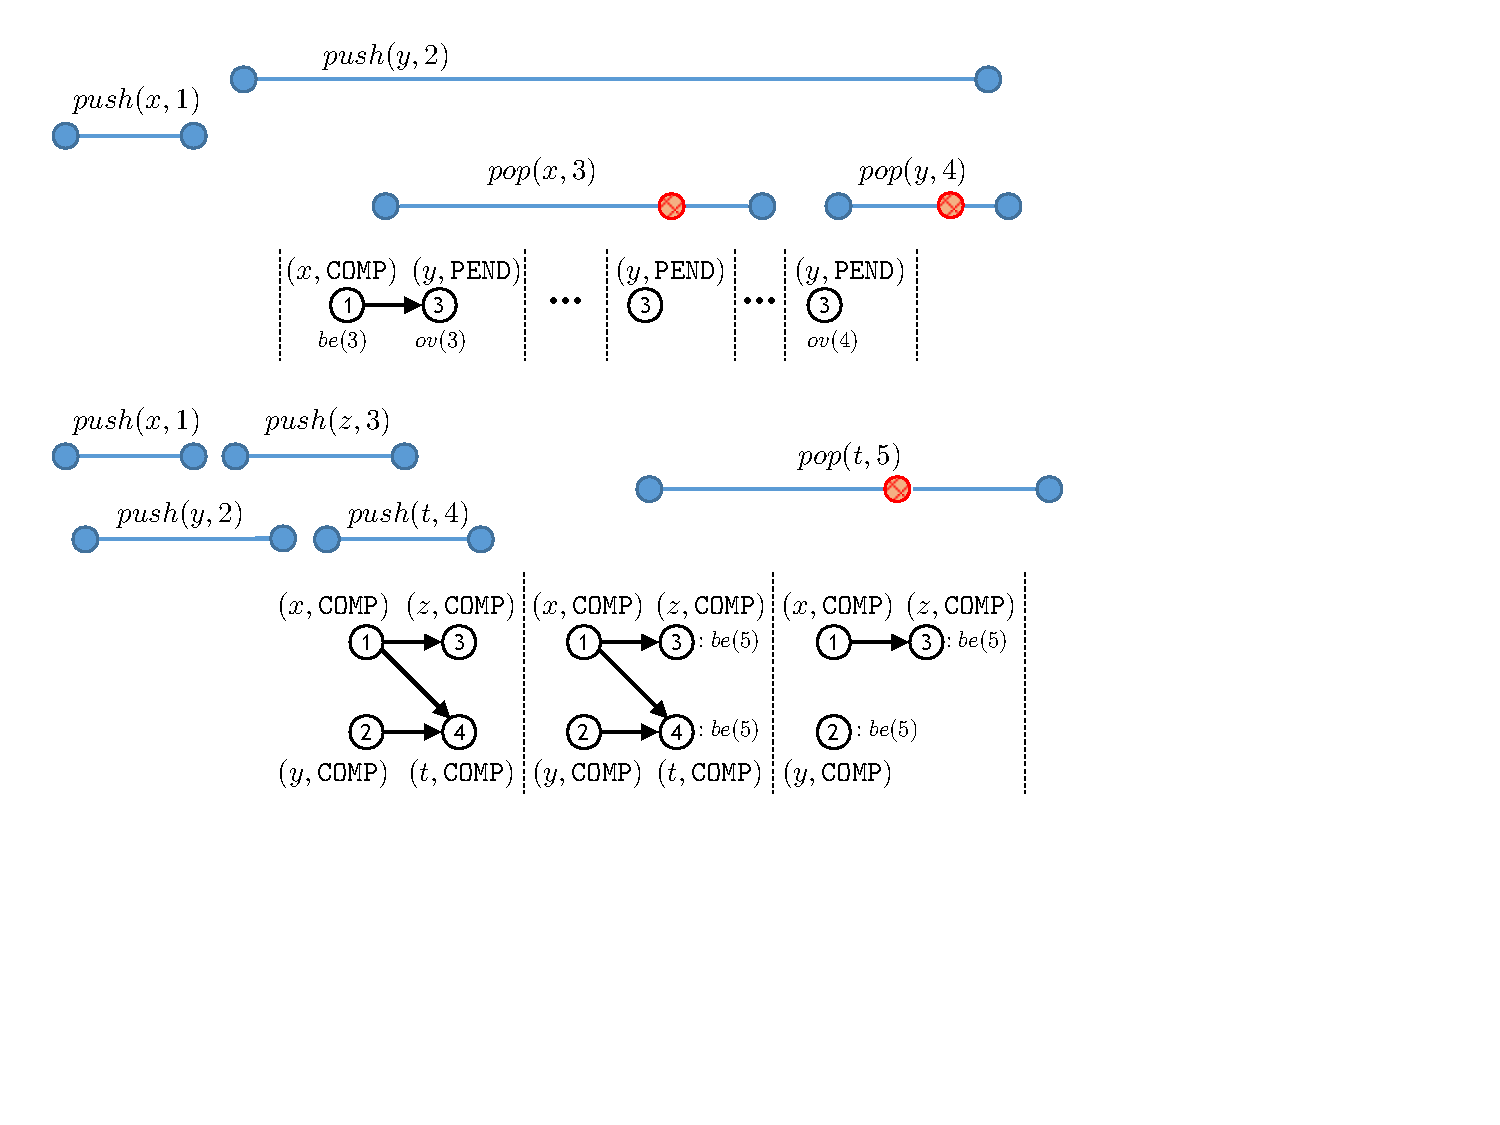
\includegraphics[width=7cm]{fig-stack.pdf}
%
%\vspace{2mm}
%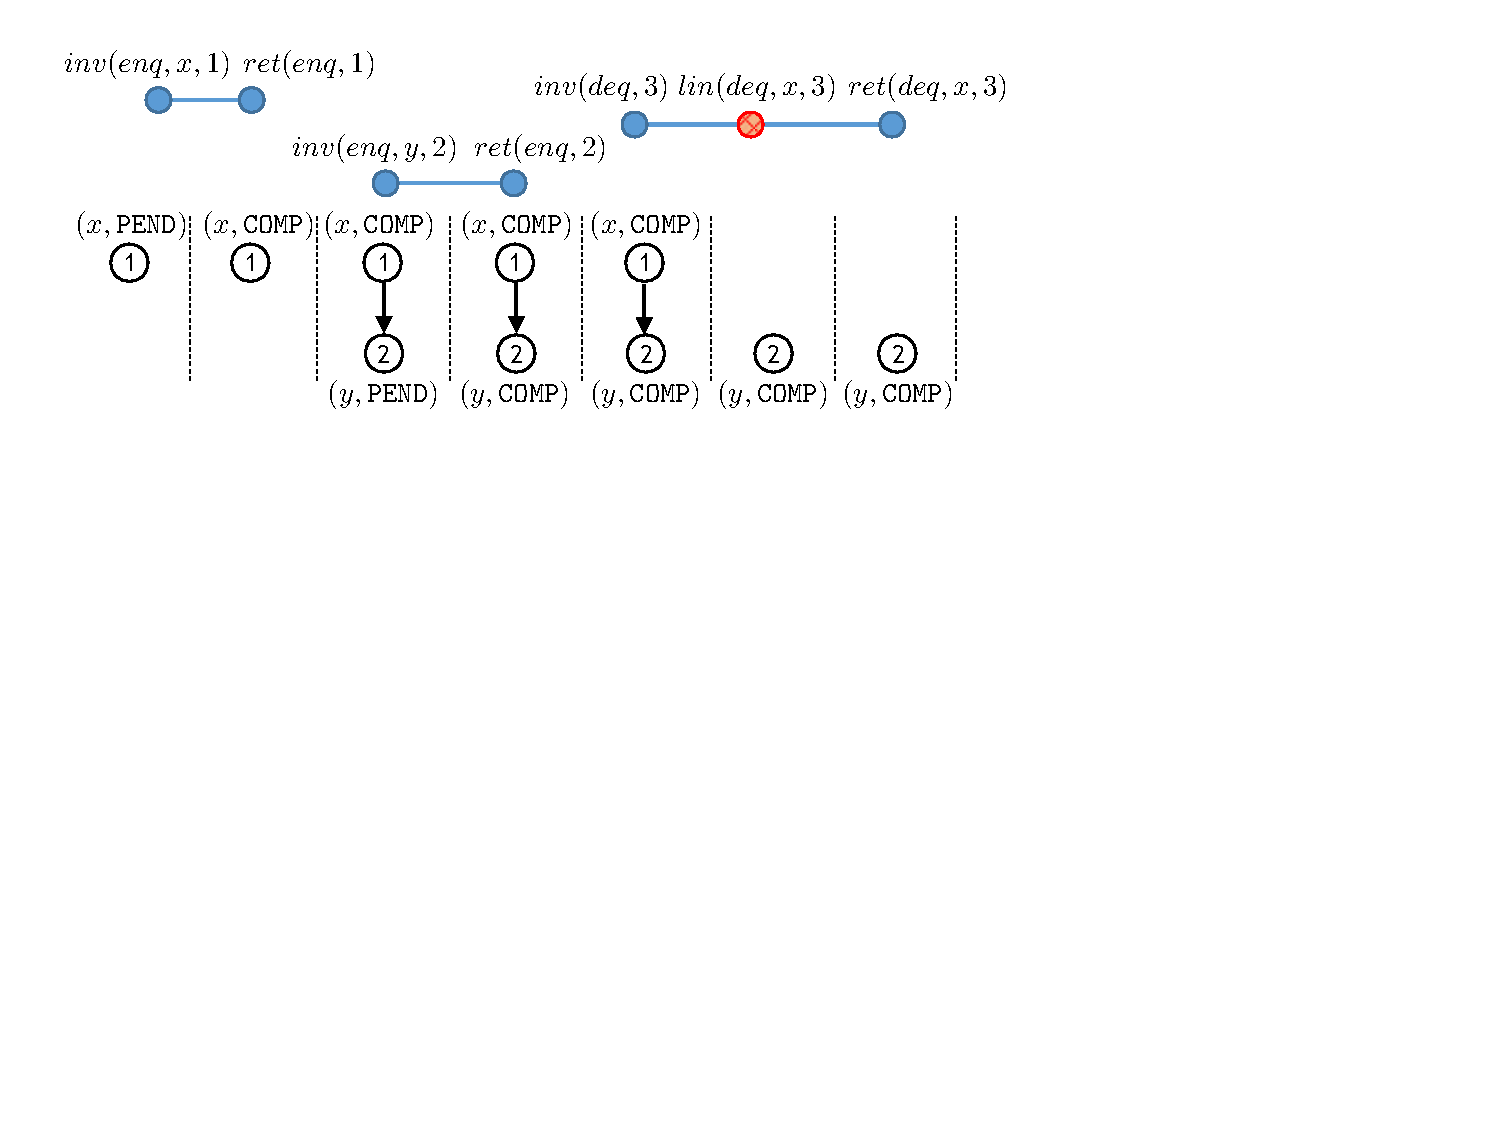
\includegraphics[width=7cm]{fig-queue2.pdf}
\vspace{-5mm}
\caption{Simulating stack histories with $AbsS$.}
\label{fig:stackSim}
\vspace{-6mm}
\end{wrapfigure}
Figure~\ref{fig:stackSim} pictures two executions of $AbsS$ for two extended histories (that include pop commit points). For readability, we give the state of $AbsS$ only after several execution prefixes delimited at the right by a dotted line. We focus on pop operations because the effect of push invocations and returns is similar to enqueue invocations and returns in $AbsQ$. Let us first consider the history in the top part of the figure. The first $AbsS$ state we give for this history is reached after the call of the pop operation with identifier $3$. This shows the effect of a pop invocation: the maximal completed pushes according to the current happens-before (in this case the push with identifier $1$) are marked as $be(3)$ (from ``before'' operation 3), and the pending pushes are marked as $ov(3)$ (from ``overlapping'' with operation 3). As a side remark, any other push operation that starts after pop $3$ would be also marked as $ov(3)$.
The commit point $com(pop,x,3)$ (pictured with a red circle) is enabled because $x$ was added by a push marked as $be(3)$. In this case, the effect of the commit point is that the push $1$ is removed from the happens-before (a more complicated case can be seen in the second execution). For the second pop, the commit point $com(pop,y,4)$ is enabled because $y$ was added by a push marked as $ov(4)$. The second execution shows an example where the marking $be(k)$ for some pop $k$ can be updated at commit points. When the two pop operations $5$ and $6$ start, the pushes $3$ and $4$ are marked as $be(5)$ and $be(6)$. Then, $com(pop,t,5)$ is enabled because $t$ was added by $push(t,4)$ which is marked as $be(5)$. Besides removing $push(t,4)$ from the state, the commit point must produce a state where a pop committing later, e.g., pop $6$, can remove $y$ which was added by a predecessor of $push(t,4)$ in the happens-before ($y$ could become the top of the stack when $t$ is removed). This history remains valid because $push(y,2)$ can be linearized after $push(x,1)$ and $push(z,3)$. Therefore, push 2, a predecessor of the push which is removed, is marked as $be(6)$. The other predecessor of the removed push, i.e., push $1$, is not marked as $be(6)$ because it happens before another push, i.e., push 3, which is already marked as $be(6)$ (the value added by push 3 should be removed as well before the value added by push 1 could become the top of the stack).

The states of $AbsS$ are tuples $\tup{O,<,\ell,rv,cp,be,ov}$ where $<$ is a strict partial order over the set $O$ of operation identifiers, $\ell: O -> \<Vals>\times\{\tt{PEND,\tt{COMP}}\}$ labels every identifier in $O$ with a value and a pending/completed flag, $rv:\<Ops> ~> \<Vals>$ records the return value of a pending pop fixed at its commit point, $cp:\<Ops> ~> \{A_1,A_2,R_1,R_2,R_3\}$ records the control point of every push ($A_1, A_2$) or pop ($R_1,R_2,R_3$) operation, $be:\<Ops> ~> 2^O$ records push operations that were maximal before a pop started or happening earlier provided that the values of all the push happening later have been removed, and $ov: \<Ops> ~> 2^O$ records push operations overlapping with a pop.
The initial state has all these components set to $\emptyset$ and the transition relation $->$ is defined in Figure~\ref{fig:transitions:AbsS}.

The transition rules which don't correspond to commit point actions are similar to those for $AbsQ$. The rule {\sc com-pop1} for $com(pop,d,k)$ is enabled only if there exists a push $k'$ which added value $d$ and which belongs to $be(k)$ or $ov(k)$. When enabled, the push $k'$ is removed from the set $O$ (and the order $<$) and for every other pop $k_1$ such that $k'$ belongs to $be(k_1)$, $k'$ is replaced in $be(k_1)$ by its predecessors for which no successor belongs already to $be(k_1)$. Also, $rv(k)$ is set to $d$. The rule {\sc com-pop1} for $com(pop,{\tt EMPTY},k)$ is enabled only if $be(k)$ is empty (i.e., all the values added by pushes ending before $k$, if any, have been removed). Then, $rv(k)$ is set to ${\tt EMPTY}$.

\begin{figure} [t]
{\scriptsize
  \centering
  \begin{mathpar}
    \inferrule[call-push]{
      k\not\in dom(cp) \\ 
      d\neq {\tt EMPTY} \\
      \forall k'.\ ov'(k') = ov(k')\cup \{k\}
    }{
      O,<,\ell,rv,cp,be,ov 
      \xrightarrow{inv(push,d,k)} 
      O\cup\{k\},<\cup\ {\tt COMP}(O)\times\{k\},\ell[k\mapsto (d,{\tt PEND})],rv,cp[k\mapsto A_1],be,ov'
    }\hspace{5mm}

    \inferrule[call-pop]{
      k\not\in dom(cp) \\
    }{
      O,<,\ell,rv,cp,be,ov
      \xrightarrow{inv(pop,k)} 
      O,<,\ell,rv,cp[k\mapsto R_1],be[k\mapsto maxCo(O)],ov[k\mapsto {\tt PEND}(O)]
    }\hspace{5mm}
    
    \inferrule[ret-pop]{
       cp(k) = R_2 \\
       rv(k)=d  
    }{
      O,<,\ell,rv,cp,be,ov
      \xrightarrow{ret(pop,d,k)}
      O,<,\ell,rv,cp[k\mapsto R_3],be,ov
    }\hspace{5mm}

    \inferrule[ret-push1]{
      cp(k) = A_1 \\
      k \in O \\
      \ell(k) = (d,{\tt PEND}) 
    }{
      O,<,\ell,rv,cp,be,ov
      \xrightarrow{ret(push,k)}
      O,<,\ell[k\mapsto (d,{\tt COMP})],rv,cp[k\mapsto A_2],be,ov
    }\hspace{5mm}
    \inferrule[ret-push2]{
      cp(k) = A_1 \\
      k \not\in O 
    }{
      O,<,\ell,rv,cp,be,ov
      \xrightarrow{ret(push,k)}
      O,<,\ell,rv,cp[k\mapsto A_2],be,ov
    }\hspace{5mm}

    \inferrule[com-pop1]{
       cp(k) = R_1 \\
       d\neq{\tt EMPTY} \\
       k'\in be(k)\cup ov(k) \\
        \ell_1(k')=d \\
       \forall k_1.\ k'\not\in be(k_1) \Rightarrow be'(k_1)=be(k_1) \\     \\
       \forall k_1.\ k'\in be(k_1) \Rightarrow be'(k_1)=(be(k_1)\setminus\{k'\})\cup \{k_2: k_2\in pred_{<}(k') \land \forall k_3. k_2<k_3 => k_3\not\in be(k_1)\} \\
    }{
      O,<,\ell,rv,cp,be,ov
      \xrightarrow{com(pop,d,k)} \\
      O\setminus \{k'\},<\uparrow k',\ell,rv[k\mapsto d],cp[k\mapsto R_2],be',ov %be[\forall k''.\ k'\in be(k'') \Rightarrow k'' \mapsto (be(k'')\cup pred_{<}(k'))\setminus\{k'\}]
    }\hspace{5mm}

    \inferrule[com-pop2]{
       cp(k) = R_1 \\
       be(k)=\emptyset
    }{
      O,<,\ell,rv,cp,be,ov
      \xrightarrow{com(pop,{\tt EMPTY},k)}
      O,<,\ell,rv[k\mapsto {\tt EMPTY}],cp[k\mapsto R_2],be,ov
    }\hspace{5mm}

    
      \end{mathpar}
  }
 \vspace{-5mm}
  \caption{The transition relation of $AbsQ$. We use the following notions: $maxCo(O)$ is the set of greatest operations in $O$ (w.r.t. $<$) which are completed, i.e., $maxCo(O)=\set{k\in O: \ell_1(k)={\tt COMP}, \forall k'\in O.\ k' < k \vee \ell_1(k')={\tt PEND}}$, ${\tt PEND}(O)=\{k\in O: \ell_2(k)={\tt PEND}\}$, and $pred_{<}(k')$ is the set of immediate predecessors of $k'$ according to $<$, i.e., $pred_{<}(k')=\set{k\in O: k < k'\land \forall k''\in O.\ k'' > k' \vee k'' < k}$.%\textcolor{red}{call-push should have $d \neq EMPTY$ in the premise. If I understand correctly, there is a problem change in $be$ in lin-pop1 rule. What I understand is we move $k''$ to every predecesoor of $k'$. But we should not move it to predecessor of $k'$ if this predecessor has a successor $m$ such that $m \in be(k'')$. Is this case reflected in your definition. Please read sub-bullet 4 of bullet 4 in the definition of $L_I$ in my document. Lin-pop2 seems ok for me. Last note: Bibliography seems not correct to me.}  $f[\forall k.\ k\mapsto expr(k)]$ is the function $g$ defined by $g(k)=expr(k)$,   $g(k)=f(k)$ for all $k$ such that $guard(k)$ is false, and 
  }
  \label{fig:transitions:AbsS}
\vspace{-6mm}
\end{figure}

Let $AbsS_0$ be the standard abstract implementation of a concurrent stack (where elements are stored in a sequence, a push operation adds atomically an element at the beginning of the sequence, and a pop operation removes atomically an element from the beginning of the sequence). For $\<Methods>=\{push,pop\}$, the alphabet of $AbsS_0$ is $C\cup R\cup Lin$.
The following result states that the library $AbsS$ has exactly the same set of histories as $AbsS_0$ (see Appendix~\ref{app:absImplStack} for a proof).

\begin{theorem}\label{th:absImplStack}
$AbsS$ is a refinement of $AbsS_0$ and vice-versa.
\end{theorem}

A trace of a queue implementation is called \emph{$Com(pop)$-complete} when every completed pop has a commit point, i.e., TODO. A stack implementation $L$ over alphabet $\Sigma$ is called \emph{with fixed pop commit points} if{f} $C\cup R\cup Com(pop)\subseteq \Sigma$ 
and every trace $@t\in Tr(L)$ is $Com(pop)$-complete.

%TODO NEEDS DATA INDEPENDENCE FOR THE COMMIT POINT TRANSITIONS TO BE DETERMINISTIC

As a consequence of Theorem~\ref{th:forSim}, $C\cup R\cup Com(pop)$-forward simulations are a sound and complete proof method for showing the correctness of a stack implementation with fixed pop commit points (up to the correctness of the commit points). 

TODO EXPLAIN THAT THIS IS DIFFERENT W.R.T. QUEUES ($Abs_0$ doesn't have commit points).

\begin{corollary}
A stack implementation $L$ with fixed pop commit points is a $C\cup R\cup Com(pop)$-refinement of $AbsS$ if{f} there exists a $C\cup R\cup Com(pop)$-forward simulation from $L$ to $AbsS$.
\end{corollary}


\subsection{A Correctness Proof For Time-Stamped Stack}

We describe a forward simulation $\mathit{fs}_2$ from $\mathit{TSS}$ to $AbsS$. Except for the constraints on the components $be$ and $ov$ of a $AbsS$ state, it is similar to the simulation $\mathit{fs}_1$ from $\mathit{HWQ}$ to $AbsQ$. Thus, the $AbsS$ states $t=\tup{O,<,\ell,rv,cp,be,ov}$ associated by $\mathit{fs}_2$ to a $\mathit{TSS}$ state $s$ satisfy the following. The set $O$ consists of all the identifiers of pushes in $s$ which didn't added yet a node to {\tt pools} or for which the input is still present in {\tt pools} (i.e., the node created by the push has {\tt taken} set to {\tt false}). A push $k$ is labeled by $(d,{\tt PEND})$ where $d$ is the input value if it's pending and by $(d,{\tt COMP})$, otherwise. 

To describe the order relation $<$ we consider the following notations: ${\tt ts}_s(k)$, resp., ${\tt TID}_s(k)$, denotes the timestamp of the node created by the push $k$ in state $s$ (the {\tt ts} field of this node), resp., the id of the thread executing $k$. By an abuse of terminology, we call ${\tt ts}_s(k)$ the timestamp of $k$ in state $s$.
Also, $k \leadsto_s k'$ when intuitively, a traversal of {\tt pools}  would encounter the node created by $k$ before the one created by $k'$. More precisely, $k \leadsto_s k'$ when ${\tt TID}_s(k) < {\tt TID}_s(k')$, or ${\tt TID}_s(k) = {\tt TID}_s(k')$ and the node created by $k'$ is reachable from the one created by $k$ in the list pointed to by ${\tt pools}[{\tt TID}_s(k)]$.
The order relation $<$ satisfies the following: (1) pending pushes are maximal, (2) $<$ is consistent with the order between node timestamps, i.e., ${\tt ts}_s(k) \leq {\tt ts}_s(k')$ implies $k'\not< k$, and (3) $<$ includes the order between pushes executed in the same thread, i.e., ${\tt TID}_s(k) = {\tt TID}_s(k')$ and ${\tt ts}_s(k) < {\tt ts}_s(k')$ implies $k < k'$.

The components $be$ and $ov$ satisfy the following constraints (their domain is the set of identifiers of pending pops):
\begin{itemize}
	\item every pop overlaps with all pending pushes, i.e., $k_1\in O$ is pending implies $k_1\in ov(k)$ for each $k, k_1$
	\item completed pushes which are maximal in $<$ are either overlapping with a pop $k$ or they were maximal in $<$ when $k$ started, i.e., every such push belongs either to $be(k)$ or $ov(k)$ for each $k$
	\item for every push that overlaps with a pop $k$ or was maximal in $<$ when $k$ started, its successors are overlapping with $k$, i.e., $k_1\in be(k)\cup ov(k)$ and $k_1 < k_2$ implies $k_2 \in ov(k)$ for each $k, k_1, k_2$
	\item $be(k)$ and $ov(k)$ don't contain predecessors of pushes from $be(k)$, i.e., $k_1 < k_2$ and $k_2 \in be(k)$ implies $k_1\not\in be(k)\cup ov(k)$ for each $k, k_1, k_2$
	\item immediate predecessors of pushes overlapping with a given pop $k$ are either overlapping with $k$ or they were maximal in $<$ when $k$ started, i.e., $k_2\in pred_{<}(k_1)$ and $k_1\in ov(k)$ implies $k_2\in be(k)\cup ov(k)$ for each $k,k_1,k_2$
	\item a pop $k$ that reached a node with timestamp $\tau$ (its variable {\tt n} points to this node) overlaps with any push that has a timestamp bigger than $\tau$ and which created a node that occurs in {\tt pools} before the node reached by $k$, i.e., ${\tt n}_s(k)={\tt n}_s(k_1)$, $k_2\leadsto_s k_1$, and ${\tt ts}_s(k_2) \geq {\tt ts}_s(k_1)$ implies $k_2\in ov(k)$, for each $k, k_1, k_2$
	\item if the variable {\tt youngest} of a pop $k$ points to a node which is not taken, then this node was created by a push in $be(k)\cup ov(k)$ or the node currently reached by $k$ is followed in {\tt pools} by another node which was created by a push in $be(k)\cup ov(k)$, i.e., ${\tt youngest}_s(k)={\tt n}_s(k_1)$, ${\tt n}_s(k_1)\text{{\tt ->taken}}={\tt false}$, and ${\tt n}_s(k)={\tt n}_s(k_2)$ implies $k_1\in be(k)\cup ov(k)$ or that there exists $k_3\in O$ such that ${\tt ts}_s(k_3) > {\tt ts}_s(k_1)$, $k_3\in be(k)\cup ov(k)$, and either $k_2\leadsto_s k_3$ or ${\tt n}_s(k_2)={\tt n}_s(k_3)$ and $k$ is traversing the last list in the array {\tt pools}, for each $k, k_1,k_2$.
\end{itemize}
Finally, for every pop operation $k$ such that ${\tt success}(k)={\tt true}$, we have that $rv(k)={\tt youngest}(k)\text{\tt->data}$. 

The proof that $\mathit{fs}_2$ is indeed a forward simulation from $\mathit{TSS}$ to $AbsS$ follows the same lines as the one given for the Herlihy\&Wing Queue. It can be found in Appendix~\ref{}.








